% !TEX root = main.tex
\section{システム構成}
\subsection{システム全体図}
本研究で構築したシステムの全体図を図\ref{fig:system_diagram}に示す.
本システムは,下位レイヤーと上位レイヤーの2つの主要な構成要素からなる.

次節以降では本研究で構成した各レイヤーのハードウェア構成およびソフトウェア構成について説明する.

\begin{figure}[h]
    \centering
    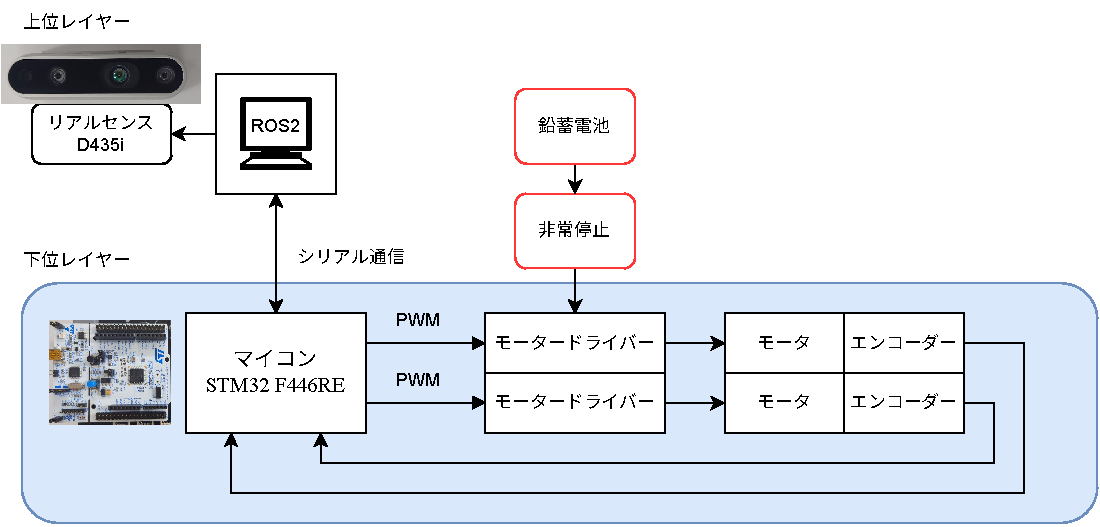
\includegraphics[width=1.0\textwidth]{figure/system.pdf}
    \caption{システム全体図}
    \label{fig:system_diagram}
\end{figure}


